\begin{refsection}
\chapter{Generic functions}\label{ch:generic}

\section{Weighted mean and outlier detection}
\label{sec:weightedmean}

\texttt{IsoplotR} uses a modified version of Chauvenet's criterion for
outlier detection. Given a set of $n$ age estimates $t = \{t_1, ...,
t_n\}$, and their standard errors $\{s[t_1], ..., s[t_n]\}$, the
conventional version of this criterion proceeds as follows:

\begin{enumerate}
\item Compute the (unweighted) arithmetic mean ($\bar{t}$) and
  standard deviation ($s[t]$) of the $n$ age determinations:
  \[
  \bar{t} = \sum_{i=1}^{n} t_i/n \mbox{~and~}
  s[t] = \sqrt{\sum_{i=1}^{n} (t_i-\bar{t})^2/(n-1)}
  \]

\item For each of the $t_i$s, compute the probability $p_i$ that
  $|\tau|>|t_i-\bar{t}|$ for
  \[
  \tau \sim \mathcal{N}(\mu=0,\sigma^2=s[t]^2)
  \]
  
\item Let $p_j \equiv \min(p_1,...,p_n)$. If $p_j<0.05/n$, then reject
  the $j$\textsuperscript{th} date, reduce $n$ by one (i.e., $n
  \rightarrow n-1$) and repeat steps 1 through 3 until all the
  surviving dates pass the third step.

\end{enumerate}

Although this procedure is effective at removing outliers in
\emph{homoscedastic} datasets, in which all datapoints are derived
from a single normal distribution, it is unable to account for
\emph{heteroscedasticity}, in which different samples are
characterised by different analytical uncertainties ($s[t_i]$ in
Equation~\ref{eq:wtdmean}). \texttt{IsoplotR} introduces a heuristic
modification to Chauvenet's criterion that detects outliers among
heteroscedastic data. For model-1 fits:

\begin{enumerate}
\item Compute the error-weighted mean of the $n$ age determinations
  $t_i$ using their analytical uncertainties $s[t_i]$ by solving
  Equation~\ref{eq:wtdmean} for $\mu$.
\item Let $\hat{\mu}$ be the maximum likelihood estimate for $\mu$ and
  let $\sigma[\hat{\mu}]$ be its standard error. For each $t_i$,
  compute the probability $p_i$ that $|\tau|>|t_i-\hat{\mu}|$ under a
  normal distribution with mean $\mu=0$ and variance $\sigma^2 = MSWD
  \times s[t_i]^2$.
\item Proceed as before.
\end{enumerate}

For a model-3 fit, the algorithm becomes:

\begin{enumerate}
\item Compute the error-weighted mean of the $n$ age determinations
  $t_i$ using their analytical uncertainties $s[t_i]$ by solving
  Equation~\ref{eq:wtdmean-model-3} for $\mu$ and $\omega$. Let
  $\hat{\mu}$ and $\hat{\omega}$ be their respective maximum
  likelihood estimates.
\item For each $t_i$, compute the probability $p_i$ that
  $|\tau|>|t_i-\hat{\mu}|$ under a normal distribution with mean
  $\mu=0$ and variance $\sigma^2=s[t_i]^2+\hat{\omega}^2$.
\item Proceed as before.
\end{enumerate}

If the analytical uncertainties are small compared to the scatter
between the dates (i.e., if $\omega \gg s[t_i]$ for all $i$ in a
model-3 fit), then this generalised algorithm reduces to the
conventional Chauvenet criterion. If, on the other hand, the
analytical uncertainties are large and the data do not exhibit any
overdispersion, then the heuristic outlier detection method is similar
to \citet{ludwig2003}'s `modified 2-sigma' approach.\\

The weighted mean calculation is accompanied by a diagram that
consists of a number of rectangular boxes (one for each date) whose
vertical position and height reflect the ages and their analytical
uncertainties, respectively (Figure~\ref{fig:wtdmeanMSWD}).  Outliers
are marked in a different colour if so requested. The weighted mean
plot offers an effective way, although arguably not \emph{the} most
effective way, to assess the dispersion of geochronological data. A
better alternative is discussed in Section~\ref{sec:radial}.

\section{Frequency distributions}
\label{sec:KDE+CAD}

Empirical cumulative distribution functions or `Cumulative Age
Distributions' (CADs) are the most straightforward way to visualise
the frequency distribution of multiple dates. A CAD is a step function
that sets out the rank order of the dates against their numerical
value:
\begin{equation}
  \mathrm{CAD}(t) = \sum_{i=1}^{n} 1(t<t_i)/n
  \label{eq:CAD}
\end{equation}

\noindent where $1(\ast) = 1$ if $\ast$ is true and $1(\ast) = 0$ if
$\ast$ is false. CADs have two desirable properties
\citep{vermeesch2007a}.  First, they do not require any pre-treatment
or smoothing of the data.  We will see that this is not the case for
all data visualisation methods. Second, it is easy to superimpose
several CADs on the same plot. This facilitates the intercomparison of
multiple samples.\\

The interpretation of CADs is straightforward but not very
intuitive. The prominence of individual age components is proportional
to the steepness of the CAD (Figure~\ref{fig:density}.a). This is
different from probability density estimates such as histograms, in
which such components stand out as peaks
(Figure~\ref{fig:density}.b). Peaks are arguably easier to identify
than inflection points and this is probably why CADs are not more
widely used as a data visualisation tool. But the ease of
interpretation of density estimates comes at a cost, as they require
smoothing and cannot as easily be combined as CADs. \texttt{IsoplotR}
implements two kinds of density estimates.\\

Histograms smooth data by binning. \texttt{IsoplotR} uses Sturges'
Rule ($\log_2[n]+1$, where $n$ is the number of data points) to
determine the default number of histogram bins, but this can be
changed to any other positive integer by the user. Alternatively,
`Kernel Density Estimates' \citep[KDEs;][]{vermeesch2012b} smooth data
by applying a (Gaussian) kernel:
\begin{equation}
  \mathrm{KDE}(t) = \sum_{i=1}^{n}\mathcal{N}\left(t | \mu=t_i,
  \sigma^2=h_i^2\right)/n
  \label{eq:KDE}
\end{equation}

\noindent where $h_i$ is the smoothing parameter or `bandwidth' of the
kernel density estimate. Using a constant value for $h_i$ across the
entire range of measurements produces a `fixed' bandwidth estimator.
If $h_i$ varies between the sample points, then KDE($t$) is known as
an `adaptive' KDE.\\

The rationale behind adaptive kernel density estimation is to use a
narrower bandwidth near the peaks of the sampling distribution (where
the ordered dates are closely spaced in time), and a wider bandwidth
in the distribution's sparsely sampled troughs. Thus, the resolution
of the density estimate is optimised according to data
availability.\\

The default bandwidth used by \texttt{IsoplotR} is calculated using
the algorithm of \citet{botev2010} and modulated by the adaptive
smoothing approach of \citet{abramson1982}, whereby:
\[
  h_i = h \sqrt{G/kde(t_i)}
  \label{eq:Abramson}
\]

\noindent in which $kde(t_i)$ is the `pilot density' using a fixed
bandwidth ($h$) evaluated at $t_i$, and $G$ is the geometric mean of
the pilot density over all the sample points \citep{kerm2003}.\\

Kernel density estimates are not to be confused with
\texttt{Isoplot}'s `probability density plots' (PDPs). The
mathematical definition of a PDP closely resembles that of the KDE,
the only difference being the substitution of the bandwidth $h_i$ by
the analytical uncertainty $s[t_i]$ in Equation~\ref{eq:KDE}. The
similarity in appearance and definition between PDPs and KDEs is the
source of much confusion.\\

The rationale behind PDPs is to emphasise the `good' data (the most
precise measurements stand out as peaks), and to reduce the prominence
of `bad' data (imprecise measurements are smoothed out by a broad
kernel). Reasonable though that might seem at first glance, this
procedure does not stand up to further scrutiny. For example, when
applied to high precision datasets, where $s[t_i]$ is very small
compared to the range of $t_i$-values, the PDP breaks down into a
sequence of spikes. Further examples and a more complete discussion of
the case against PDPs are presented by \citet{vermeesch2012b,
  vermeesch2018b}.\\

This discussion leaves us with one question: if PDPs are not a valid
data visualisation tool, then how should one account for the
heteroscedasticity of geochronological data?  \texttt{IsoplotR}
implements two alternative options. The first of these is the weighted
mean plot (Section~\ref{sec:weightedmean}).  Although this diagram
does show both the individual age estimates and their analytical
uncertainties, it is not very effective at revealing components of
clustered ages, especially in large ($n>50$, say) datasets. The second
option is the radial plot, which is discussed in
Section~\ref{sec:radial}.\\

\section{Radial plots}
\label{sec:radial}

The radial plot is a graphical device that was specifically designed
to display heteroscedastic data, and is constructed as follows.
Consider the usual set of dates $t_i$ and uncertainties $s[t_i]$ (for
$1 \leq i \leq n$); define $z_i = z(t_i)$ to be a transformation of
$t_i$; and let $s[z_i]$ be its propagated analytical uncertainty.
For example,
\begin{equation}
  \begin{cases}
  \phantom{s[}z_i\phantom{]}\! & \! = \ln[t_i]\\
  s[z_i]\! & \! = s[t_i]/t_i
  \end{cases}
  \label{eq:logtransform}
\end{equation}

\noindent in the case of a logarithmic transformation. Then the radial
plot is a scatter plot of $(x_i,y_i)$ values, where
\begin{equation}
  \begin{split}
    x_i & = 1/s[z_i] \\
    \mbox{and~} y_i & = \frac{z_i-z_\circ}{s[z_i]}
  \end{split}
  \label{eq:radial}
\end{equation}

\noindent in which $z_\circ$ is some reference value such
as the mean. The slope of a line connecting the origin of this scatter
plot with any of the $(x_i,y_i)$s is proportional to $z_i$ and, hence,
a function of the date $t_i$.\medskip

It is helpful to draw a radial scale at some convenient distance from
the origin and annotate it with labelled ticks at the appropriate
angles. While the angular position of each data point represents the
date, its horizontal distance from the origin is proportional to the
precision. Imprecise measurements plot on the left-hand side of the
radial plot, whereas precise age determinations are found further
towards the right. Thus, radial plots allow the observer to assess
both the magnitude and the precision of quantitative data in one
glance:

\begin{center}
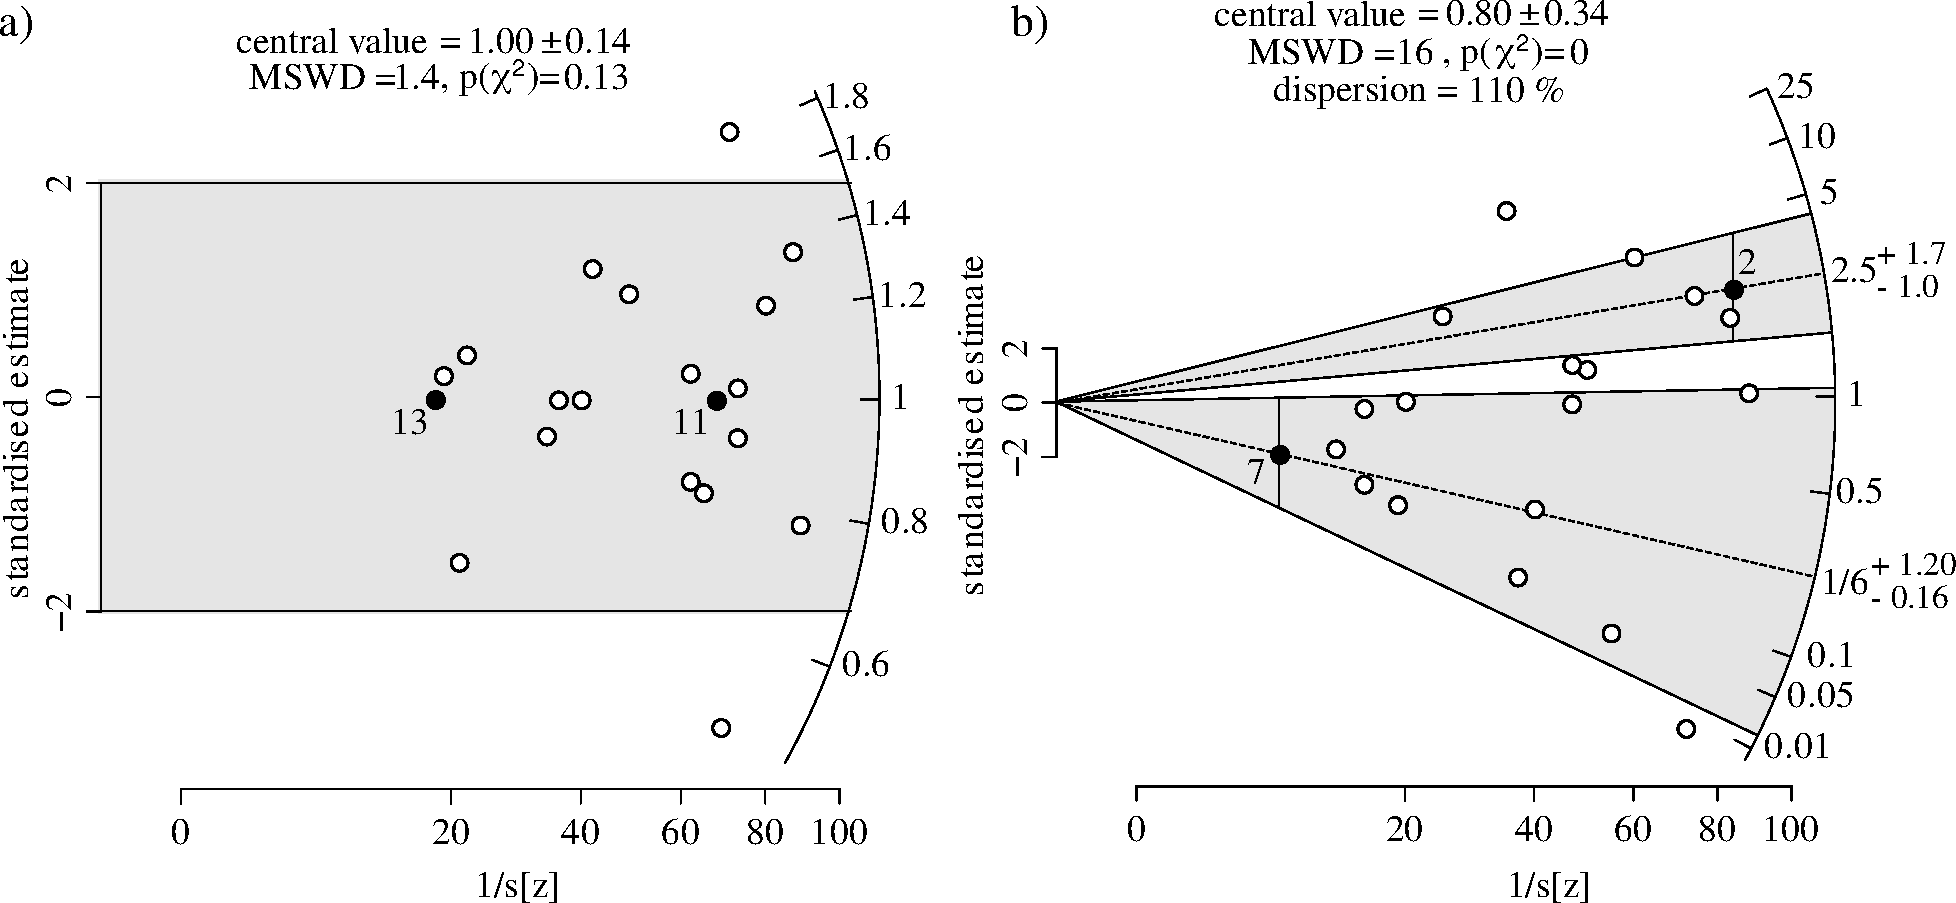
\includegraphics[width=.9\textwidth]{../figures/radial.pdf}
\end{center}
\begingroup \captionof{figure}{Radial plots for two synthetic datasets
  from \citet{vermeesch2018d}.  a) approximately 95\% of the samples
  in the first dataset plot within a symmetric `2-sigma' band around
  the origin. These data are therefore compatible with a single
  homogeneous population, and pass the chi-square test.  b) the age of
  each aliquot can be obtained by projecting the corresponding scatter
  point onto the radial scale.  Projecting a `2-sigma' error bar onto
  the same scale yields the 95\% confidence intervals of $t_2 = 2.5
  +1.7/-1.0$ and $t_{7} = 0.17 +1.20/-0.16$. The second sample does
  not fit within a `2-sigma' band, and is more adequately described by
  a random effects model with two parameters: the central ratio and
  the dispersion.\\}
  \label{fig:radial}
\endgroup

Radial plots are widely used in fission track and luminescence dating
\citep{galbraith1990a, galbraith1999}, but are yet to find their way
into other branches of geochronology. \texttt{IsoplotR} generalises
this valuable tool to all types of geochronological data.  In addition
to being an effective way to visualise heteroscedastic data, the
radial plot also represents a convenient vehicle for further data
interpretation and modelling, as will be discussed
Section~\ref{sec:mixtures}.\\

\noindent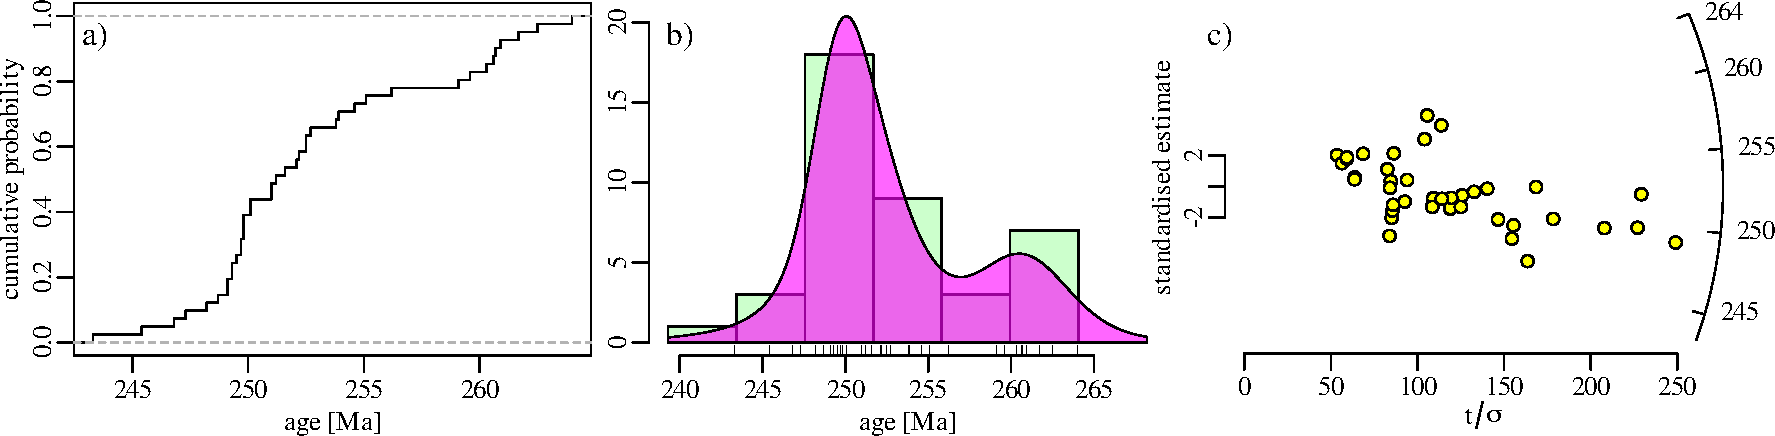
\includegraphics[width=\textwidth]{../figures/frequency.pdf}
\begingroup \captionof{figure}{a) CAD, b) histogram/KDE and c) radial
  plot of the same dataset \citep[from][]{ludwig2003}. }
\label{fig:density}
\endgroup

\section{Mixture models}
\label{sec:mixtures}

The weighted mean algorithm outlined in Sections~\ref{sec:mswd} and
\ref{sec:weightedmean} assumes that geochronological data obey normal
statistics. This assumption may be approximately correct for high
precision datasets but must inevitably be incorrect for low precision
ones.\\

Geologic time is a strictly positive quantity that is incompatible
with the symmetric Gaussian bell curve, which is defined over the
range of values from $-\infty$ to $+\infty$. Because geochronological
datasets must be strictly positive, their uncertainty distributions
must be asymmetric, with skewness being inversely proportional to
precision. This asymmetry is removed by the logarithmic transformation
that is used to construct radial plots
(Equation~\ref{eq:logtransform}), and which can also be applied to
KDEs:\\

\noindent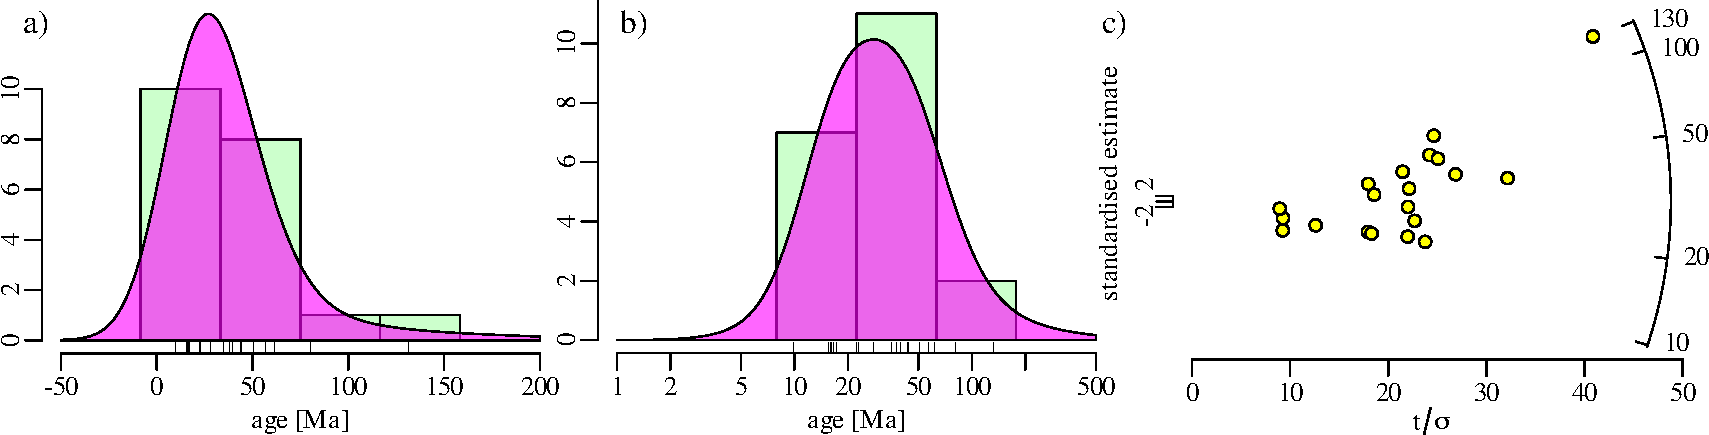
\includegraphics[width=\textwidth]{../figures/logtrans.pdf}
\begingroup
\captionof{figure}{Young U--Pb carbonate dates shown a) on a linear
  scale, whose KDE spills over into nonsensical negative data space,
  and b) on a logarithmic scale, which fixes this problem. c) shows
  the same data as a radial plot with a logarithmic time scale.\\}
\endgroup

We can reformulate Equation~\ref{eq:wtdmean} in terms of the
transformed variables $z_i$:
\begin{equation}
  p(z_i|\mu,\omega) = \mathcal{N}\left( \mu, \sigma^2 =
  s[z_i]^2+\omega^2 \right)
  \label{eq:central}
\end{equation}

\noindent which can be solved by the method of maximum likelihood as
before, yielding two estimates $\hat{\mu}$ and $\hat{\omega}$. The
\textbf{central age} is defined as $\exp(\hat{\mu})$, and
$\hat{\omega}$ represents the (over)dispersion of the data.  This is a
relative quantity (due to the log-transform) that estimates the
\texttt{coefficient of variation} ($=\sigma/\mu$) of the true ages. The
difference between the central age and the weighted mean age is
usually small unless the data are imprecise and/or strongly
overdispersed. In those cases, the central age yields the geologically
most meaningful value.\\

\noindent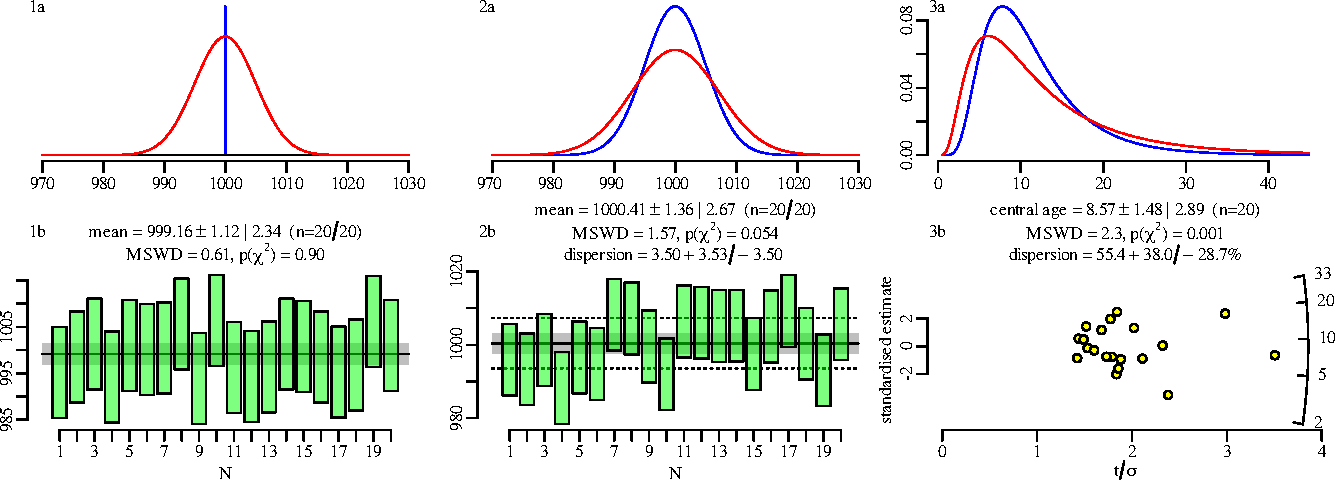
\includegraphics[width=\textwidth]{../figures/3means.pdf}
\begingroup \captionof{figure}{Three different age models implemented
  in \texttt{IsoplotR}. 1a) If the true age is a discrete event (blue
  peak at 1000~Ma), and the analytical uncertainties follow a normal
  distribution with zero mean and 5~Ma standard deviation, then the
  predicted distribution of the dates (red line) is a normal
  distribution with mean at 1000~Ma and a 5~Ma standard deviation. 1b)
  In this case the ordinary weighted mean (Equation~\ref{eq:wtdmean})
  is the most appropriate estimator of the true age. 2a) If the true
  age is drawn from a normal distribution with a mean of 1000~Ma and a
  standard deviation of 5~Ma (blue line), and if the analytical
  uncertainties follow a normal distribution with zero mean and 5~Ma
  standard deviation, then the predicted distribution of the dates
  (red line) is a normal distribution with mean at 1000~Ma and a
  $\sqrt{50}$~Ma standard deviation. 2b) In this case the random
  effects model of Equation~\ref{eq:wtdmean-model-3} is the most
  appropriate estimator of the mean \emph{and} the standard deviation
  of the true ages. The latter parameter is reported as the dispersion
  in the legend. 3a) If the true ages are drawn from a lognormal
  distribution with location parameter $\exp[\mu]=10$~Ma and
  dispersion parameter $\sigma/\mu=50$\% (blue line), and the
  analytical uncertainties are $\sim$50\%, then the distribution of
  the measured dates (red line) is a lognormal distribution with
  $10/\sqrt{2}$\% dispersion parameter. 3b) In this case the random
  effects model of Equation~\ref{eq:central} is the best way to
  average the data, and the radial plot with logarithmic scale is the
  best way to visualise the results. Note that the dispersion is
  reported in absolute units on the weighted mean plot (panel b), and
  in relative units on the radial plot (panel c).\\} \endgroup

The random effects model represented by Equation~\ref{eq:central} is
referred to as a \textbf{continuous mixture} model. It assumes that
the overdispersion of the data is caused by a continuous process that
yields a (log)normal distribution of true ages. As previously
mentioned in Section~\ref{sec:overdispersion}, one example of such a
process is the fractional crystallisation of plutons, which may take
hundreds of thousands of years, resulting in a range of zircon U-Pb
ages. A second example is the gradual cooling of tectonic blocks
during exhumation, which may cause the fission track system in
compositionally heterogeneous apatite populations to `close' at
different times. However, such continuous processes are by no means
the only cause of overdispersion in geochronology.\\

Consider, for instance, a detrital mixture originating from two or
more differently aged sources. Such a \textbf{discrete mixture} is
more adequately described by the following equation:
\begin{equation}
  \mathcal{LL}({\boldsymbol\mu},{\boldsymbol\pi}|\mathbf{z},\mathbf{s[z]}) =
  \sum_{i=1}^n\ln\!\left[\sum_{j=1}^k \pi_j \mathcal{N}\left( z_i | \mu_j, s[z_i]^2\right)\right]
  \label{eq:mixture}
\end{equation}

\noindent where ${\boldsymbol\mu}=\{\mu_1,\ldots,\mu_k\}$,
${\boldsymbol\pi}=\{\pi_1,\ldots,\pi_k\}$,
$\mathbf{z}=\{z_1,\ldots,z_k\}$,
$\mathbf{s[z]}=\{s[z_1],\ldots,s[z_k]\}$, $k$ is the number of
components, $\mu_j$ is the mean of the $j$\textsuperscript{th}
component (so that $\exp[\mu_j]$ is the corresponding age), and
$\pi_j$ is the proportion of the population that belongs to the
$j$\textsuperscript{th} component. Equation~\ref{eq:mixture} comprises
$n$ measurements and $2k-1$ unknowns ($\mu_j$ and $\pi_j$ for $1 \leq
j \leq k$ with $\pi_k=1-\sum_{j=1}^{k-1}\pi_j$). It can be solved by
the method of maximum likelihood.\\

\noindent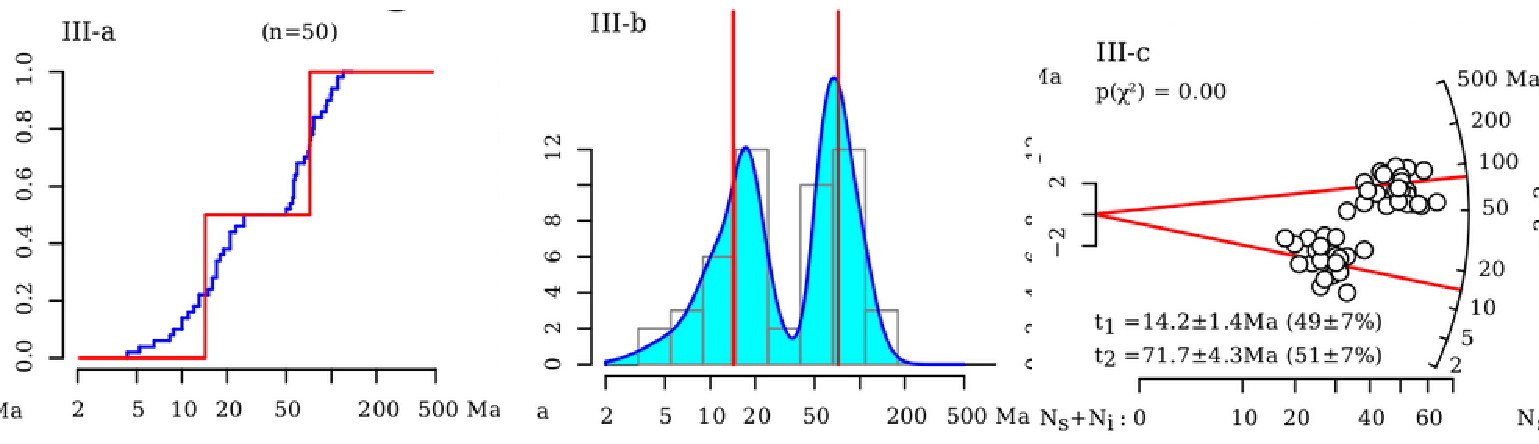
\includegraphics[width=\textwidth]{../figures/discretemixtures.pdf}
\begingroup \captionof{figure}{a) cumulative distribution of the true
  ages of a binary mixture of two discrete age components (red) and
  the CAD of the measured ages of 50 measured dates (blue). b)
  histogram and KDE of the binary mixture. c) results of the mixture
  model, shown as a radial plot.\\}
\label{fig:discretemixtures}
\endgroup

Choosing the right number of components ($k$) is a problem that merits
further discussion. \texttt{IsoplotR} implements the Bayes Information
Criterion (BIC) as a way to automatically pick the `optimal' value of
$k$ for any given dataset \citep[Section~5.6 of][]{galbraith2005}. But
this option should be used with caution because, for real datasets,
the number of components always increases with sample size. This
happens because the power of Equation~\ref{eq:mixture} to resolve even
the smallest degree of overdispersion increases with sample size.\\

Suppose that one uses the youngest component in a discrete mixture
model to estimate the maximum depositional age of a sedimentary
sequence. Then the resulting value would never converge to a specific
value.  Instead, one would find this minimum age to drift to ever
younger values until a point where the youngest age component in a
large dataset becomes younger than the actual depositional age. In
most cases it is, therefore, best to resist the temptation to use the
automatic peak fitting option. It is better to choose a specific
number of components instead, based on geological considerations.\\

\noindent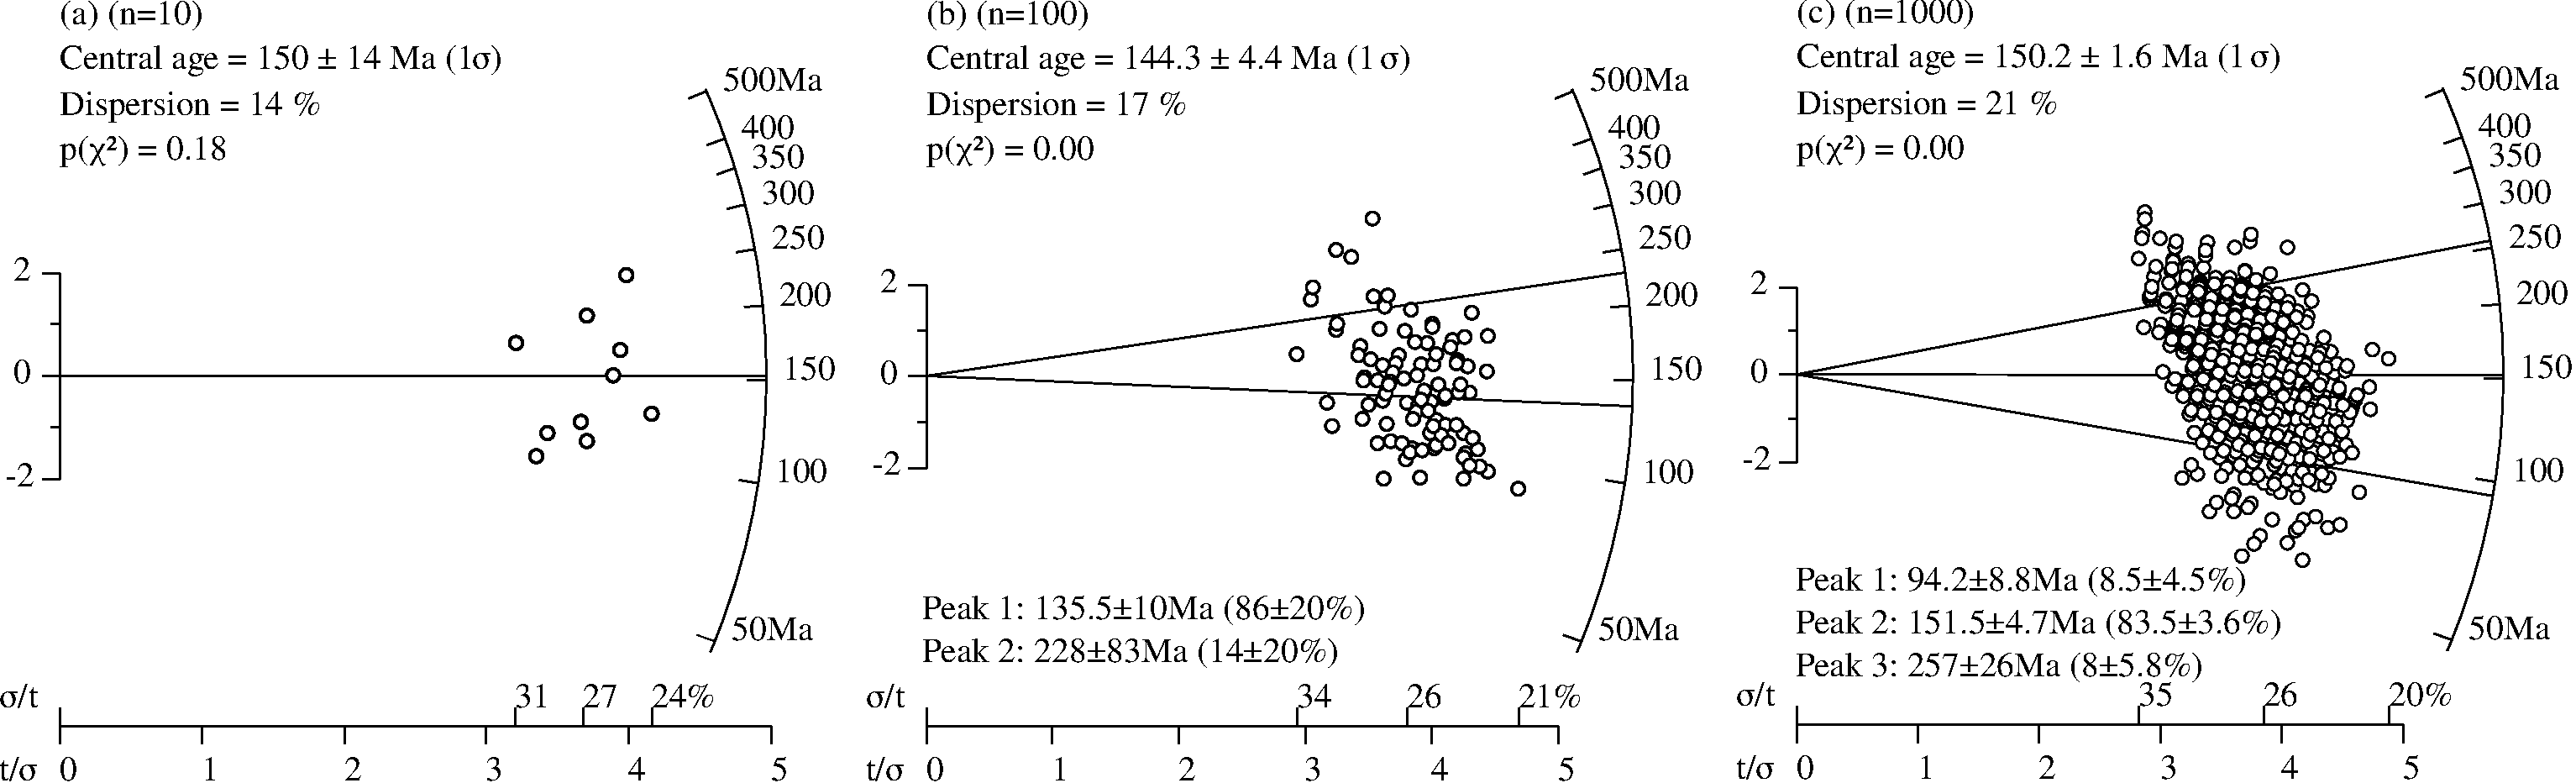
\includegraphics[width=\textwidth]{../figures/increasingn.pdf}
\begingroup \captionof{figure}{Application of finite mixture modelling
  to a continuous mixture. Increasing sample size from left (a) to
  right (c) provides statistical justification to fit more
  components. Note that the age of the youngest age component gets
  progressively younger with increasing sample size, from 150~Ma for
  sample (a) to 94~Ma for sample (c), and is therefore not a reliable
  estimator of the minimum age. Figure adapted from
  \citet{vermeesch2019b}.\\}
\label{fig:increasingn}
\endgroup

If one is mainly interested in the youngest age component, then it is
more productive to use an alternative parameterisation, in which all
grains are assumed to come from one of two components, whereby the
first component is a single discrete age peak ($\exp[\gamma]$, say)
and the second component ($\exp[\mathcal{N}'(z|\mu,\omega^2)]$ where
$\mu<\gamma$) is a continuous distribution such as
Equation~\ref{eq:central}, but truncated at this discrete value:
\begin{equation}
  \mathcal{LL}(\pi,\gamma,\mu,\omega|\mathbf{z},\mathbf{s[z]}) =
  \sum\limits_{j=1}^{n} \ln\!\left[
    \pi \mathcal{N}(z_i|\gamma,s[z_i]^2) +
    (1-\pi) \mathcal{N}'(z_i|\mu,s[z_i]^2+\omega^2)
    \right]
\label{eq:Lminagemod}
\end{equation}

One caveat is that, if this minimum age model is applied to relatively
small and/or high precision datasets such as most U-Pb measurements,
then the minimum age estimate will simply be equal to the youngest
date.  It is only for large and/or low precision datasets (such as
fission tracks), that the minimum age estimate will be older than then
youngest grain.  Crucially, this value will not drift to smaller
values with increasing sample size, but will converge to a distinct
minimum age.\\

\noindent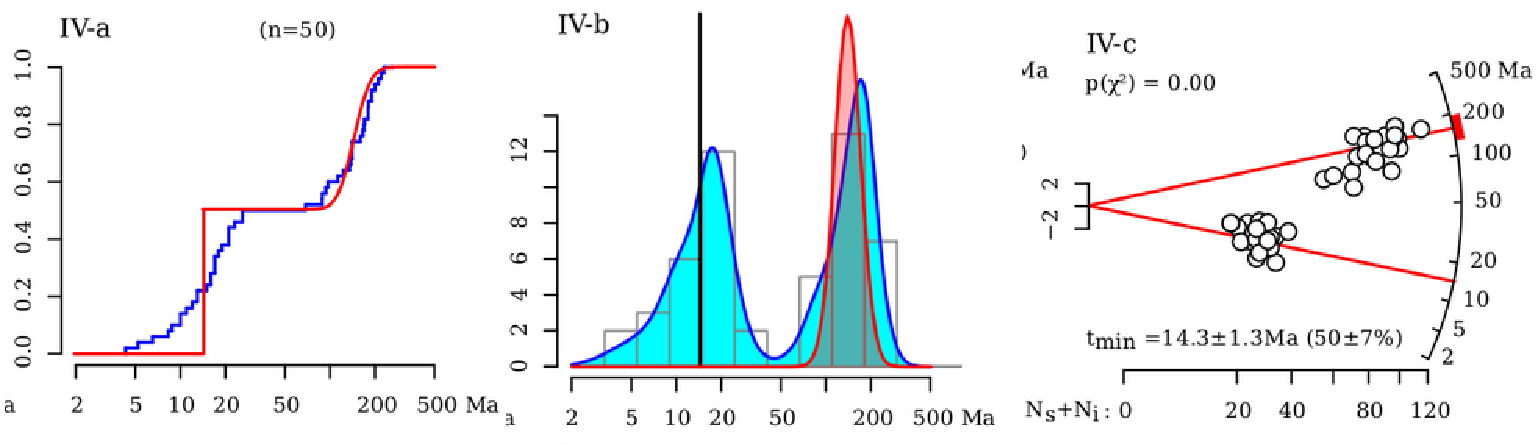
\includegraphics[width=\textwidth]{../figures/minagemod.pdf}
\begingroup \captionof{figure}{A binary mixture combining discrete and
  continuous age components shown as a) CADs and b) histograms and
  KDEs, with the true age components shown in red, and the measured
  age distribution in blue. c) radial plot with the minimum age model
  of Equation~\ref{eq:Lminagemod}.}
\label{fig:minagemod}
\endgroup

\printbibliography[heading=subbibliography]

\end{refsection}
